Nella fase 2 si svolgeranno le seguenti attività:
\begin{itemize}
	\item normazione: modifiche alle \textit{Norme di progetto} secondo quanto segnalato alla Revisione dei requisiti. Si procede poi con il suo incremento;
	\item pianificazione della qualifica: modifiche al \textit{Piano di qualifica} secondo quanto segnalato alla Revisione dei requisiti. Si procede poi con il suo incremento;
	\item pianificazione delle attività: modifiche al \textit{Piano di progetto} secondo quanto segnalato alla Revisione dei requisiti;
	\item analisi dei requisiti: modifiche al \textit{Analisi dei requisiti} secondo quanto segnalato alla Revisione dei requisiti;
	\item progettazione PoC e Technology Baseline: vengono ricercate le tecnologie, i framework e le librerie ritenute più adatte allo sviluppo del prodotto;
	\item codifica: realizzazione del PoC;
	\item verifica per il colloquio: verifica del PoC in vista di una discussione Agile con il committente;
	\item colloquio: viene effettuato il colloquio con la committente;
	\item incremento progettazione e codifica: in base alla segnalazioni ricevute durante il colloquio con il committente vengono eseguite opportune modifiche;
	\item incremento della pianificazione delle attività: viene aggiornato il \textit{Piano di progetto} con il consuntivo riguardante la fase 2;
	\item verifica per la consegna: vengono verificati tutti i documenti e la Technology Baseline con la relativa codifica;
	\item consegna del materiale in ingresso;
	\item preparazione alla presentazione.
\end{itemize}

\begin{figure}[h]
	\centering
	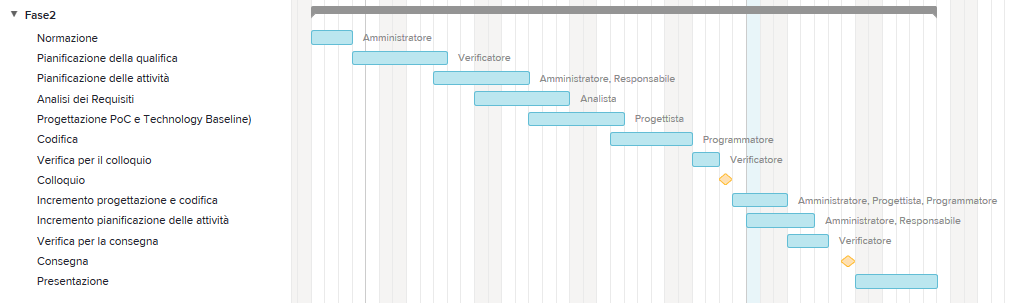
\includegraphics[scale=0.67]{images/fase2.png}
	\caption{Diagramma di Gantt riguardante la fase 2}
\end{figure}